\subsection{Explicación de los gráficos}

En los experimentos hechos se realizaron distintos tipos de gráficos

\begin{itemize}
	\item Un gráfico que contiene, en un eje, el promedio de los tiempos totales
	a cada gateway (puntos y lineas rojas), junto con barras verticales rojas
	para indicar la desviación estandar que tuvo esa muestra. A su vez, en el
	mismo grafico, en otro eje, los valores normalizados $Z_{i}$ (ver
	\ref{eq:z}) de cada enlace segun fueron calculados en la metodología y una
	barra horizontal situada en el valor de la tabla $t$ para ese tamaño de
	muestra.  Por encima de este umbral son clasificados los enlaces como
	intercontinentales por el método presentado en este trabajo.  Para
	facilitar la lectura se coloreó con naranja los enlaces que sean
	intercontinentales segun el método propuesto.

	\item Una tabla con las ciudades y paises de donde se localizan las IPS,
	una por cada servicios de geolocalización de IPS para así poder comparar
	los errores cometidos por estos servicios segun el criterio de
	determinación propuesto en este trabajo de los dos tipos de enlaces.

	\item Un mapa con las coordenas por cada servicios de geolocalización de
	IPS ($plotip$ y $geoiptool$) para poder visualizar y contrastar estos
	enlaces desde otra perspectiva que no sean los tiempos de enlace y que
	se complemente con la tabla antes mencionada.
\end{itemize}

Ademas para obtener un resultado estadistico consistente a lo largo de todas las
experimentaciones, para cada TTL se realizaron 30 muestras.

\clearpage

\subsection{Universidad de La Habana}

En este experimento analizaremos como se comportan los paquetes enviados hasta
la web de la Universidad de La Habana\footnote{http://www.uh.cu/}. Al momento
de realizarse el experimento, su IP es 200.55.139.216.

\subsubsection{Round Trip Times}

\begin{figure}[ht]
	\begin{center}
		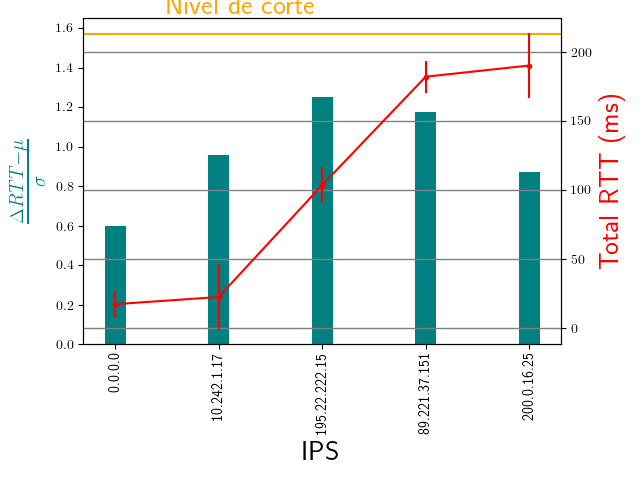
\includegraphics[width=0.8\columnwidth]{imagenes/rtts_habana.png}
		\caption{Grafico de RTTS totales y de enlaces para la Universidad de La Habana}
	\end{center}
\end{figure}

El largo de la ruta es de 5 y no hubo casos en los que para un TTL no respondiera
Time Exceeded o Echo Replay. Adem\'as, podemos observar que ningun cable es considerado
transatlantico, utilizando el algoritmo expuesto anteriormente, si bien se
puede ver una diferencia considerable de RTT en la IP 195.22.222.15 y
89.221.37.151.  \\

\subsubsection{Posiciones geográficas}

Haremos un mejor an\'alisis utilizando geolocalizaci\'on para intentar entender
el camino del paquete. Tanto geoiptool como plotip nos dan dos caminos bastante
distintos como muestran las tablas a continuaci\'on

\begin{figure}[ht]
	\begin{subfigure}[b]{0.5\textwidth}
		\centering
		\begin{tabular}{|c|c|c|}
	\hline
	IP & Ciudad & Pais \\
	\hline
	10.242.1.17 & Aachen & Alemania \\
	\hline
	195.22.222.15 & Chicago & Estados Unidos  \\
	\hline
	89.221.37.151 &  & Grecia \\
	\hline
	200.0.16.25 & La Habana & Cuba \\
	\hline
\end{tabular}

		\caption{PlotIP}
	\end{subfigure}
	\begin{subfigure}[b]{0.5\textwidth}
		\centering
		\begin{tabular}{|c|c|c|}
	\hline
	IP & Ciudad & Pais \\
	\hline
	10.242.1.17 & &  \\
	\hline
	195.22.222.15 & & Italia  \\
	\hline
	89.221.37.151 & & Italia \\
	\hline
	200.0.16.25 & & Cuba \\
	\hline
\end{tabular}

		\caption{GeoIPTool}
	\end{subfigure}
	\caption{Ciudades y Paises de las IP's usando PlotIP/GeoIPTool para la Universidad de La Habana}
\end{figure}


Primero vemos que en plotip tiene poco sentido el camino de ir de Alemania a
Estados Unidos a Grecia para luego volver a Cuba, adem\'as de que no se condice
con los RTTs medidos. Al no poder ser procesada la IP 10.242.1.17 por geoiptool
nos hace pensar que el caso de Alemania puede estar mal. Con esto en mente, lo
mas factible viendo los resultados de plotip es el camino Buenos Aires -
Estados Unidos - Cuba. Descartamos Grecia porque creemos que no tiene sentido
hacer ese trayecto por la localizaci\'on tan cercana de Cuba a Estados
Unidos.\\

En geoiptool, nos da un camino que puede ser valido ya que es ir a Italia para
luego ir a Cuba. Si bien la distancia de Buenos Aires a Estados Unidos es tan
grande como la que separa a algunos continentes, resulta raro que no haya
detectado ningun camino intercontinental nuestro algoritmo. Esto nos hace ver
como mas posible entre ambos caminos el primero. Igualmente es posible que el
nivel de corte calculado con el metodo de Cimbala sea muy grande en este
caso.\\

Presentamos los graficos generados utilizando la localizaci\'on provista por
ambas herramientas para poder comparar visualmente los recorridos.

\begin{figure}[ht]
	\begin{subfigure}[b]{0.5\textwidth}
		\centering
		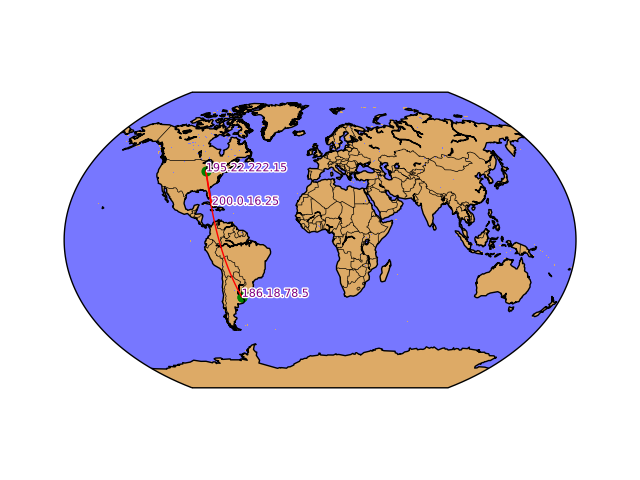
\includegraphics[width=\linewidth]{imagenes/mapa_habana_plotip.png}
		\caption{PlotIP}
	\end{subfigure}
	\begin{subfigure}[b]{0.5\textwidth}
		\centering
		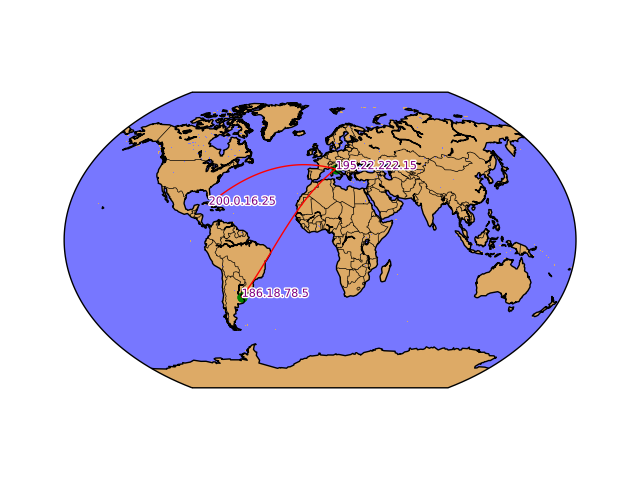
\includegraphics[width=\linewidth]{imagenes/mapa_habana_geoip.png}
		\caption{GeoIPTool}
	\end{subfigure}
	\caption{Mapas generados a partir de las IP's usando PlotIP/GeoIPTool para la Universidad de La Habana}
\end{figure}

Por ultimo, en caso de que la verdadera ruta haya sido la que pasa por EEUU, entonces
nuestro algoritmo dio un 100\% de acierto. Pero, si la ruta resulta ser la que pasa
por Italia, entonces tendremos un falso negativo. En ese caso, para solucionarlo, podriamos
usar un nivel de corte de aproximadamente 1.2.

\subsection{Red de Tecnología Australiana}

En este experimento se observo el trayecto que nos devuelve la herramienta de \textit{traceroute} para \url{http://www.atn.edu.au/}, la página de la Red de Tecnología Australiana que compone un total de 5 universidades, y cuya IP es 130.220.0.127 (al menos al momento de la presente experimentación). Como resultado pudimos trazar una ruta de 24 HOPs, de los cuales la mayoria no tienen representación en los graficos. Esto se debe a dos razones, la primera es que para 5 de los TTL's (aproximadamente el 20\%) obtuvimos un Time Exceeded. La otra razon es que para 8 de los TTL's (aproximadamente el 42.11\%) el cálculo del $\Delta RTT$ nos devolvio un valor negativo, y por ende los descartamos conciderandolos como parte del enlace, y no como un nodo del trayecto. No obstante los 11 restantes HOPs fueron suficiente para obtener una idea del camino aproximado.

\subsubsection{Posiciones geográficas}

Al igual que en el caso anterior, para esta experimentación se intento darle una referencia geografica aproximada a cada uno de los salto no descartados. Para esto acudimos a dos servicios de geolocalización de IPs, PlotIP y GeoIPTool. Ambos servicios sugirieron para cada IP una ubicación aproximadamente parecida para la mayoria de las IPs, o por lo menos siempre coincidieron en el pais de alocación de cada una, no obstante hubo algunas discrepancias. Por ejemplo para la IP 64.125.13.241 el servicio de PlotIP la localiza en New York, y GeoIPTool en Louisville, que según los mapas geograficos mantienen una buena distancia. Pensamos que esto se debe a que quizas simplemente alguno de los dos esta mas actualizado. También hubo diferencias con respecto a la geolocalización de las IPs de Australia, a varias PlotIP las localiza en Wahroonga y GeoPlotIP en Canberra, aunque a diferencia del caso anterior no hay tanta distacia entre ambas ciudades. El único caso particular en Australia es el de la IP 202.158.194.161, en donde claramente Perth guarda una distancia no despreciable con respecto a Surry Hills.

Mas alla de las mencionadas discrepancias, de ambos servicios pudimos estimar una ruta bastante clara con respecto a los paises visitados. Desde el pais de origen (Argentina), se hizo un salto de larga distancia a Estados Unidos, para luego partir finalmente a Australia, por lo que suponemos algun cable submarino. Si bien el desvio de Argentina a Estados Unidos resulta en un trayecto geograficamente mucho mas largo que el de la mínima distacia de Argentina a Australia, lo contemplamos como un resultados bastante esperable al contrastarlo con el mapa de cables intercontinentales, ya que la gran mayoria de ellos en América salen de Estados Unidos, y no parece haber ninguna ruta mas directa hacia Australia. Por ende los mapas realizados para los datos provenientes de ambos servicios resultaron muy similares. Las unicas pequeñas desviaciones son las que supusieron las discrepancias del caso de New York-Lousville, y Surry Hills-Perth explicados anteriormente.

\begin{figure}[ht]
	\begin{subfigure}[b]{0.5\textwidth}
		\centering
		\begin{tabular}{|c|c|c|c|}
	\hline
	TTL & IP & Ciudad & Pais \\
	\hline
	7 & 200.89.160.13 & Quilmes & Argentina \\
	\hline
	10 & 67.17.99.233 &  & Estados Unido \\
	\hline
	12 & 4.69.209.173 &  & Estados Unido \\
	\hline
	13 & 64.125.13.241 & New York & Estados Unido \\
	\hline
	17 & 202.158.194.161 & Surry Hills & Australia \\
	\hline
	18 & 113.197.15.156 & Wahroonga & Australia \\
	\hline
	20 & 113.197.15.9 & Wahroonga & Australia \\
	\hline
	21 & 113.197.15.29 & Wahroonga & Australia \\
	\hline
	22 & 138.44.192.25 &  & Australia \\
	\hline
\end{tabular}

		\caption{PlotIP}
	\end{subfigure}
	\begin{subfigure}[b]{0.5\textwidth}
		\centering
		\begin{tabular}{|c|c|c|c|}
	\hline
	TTL & IP & Ciudad & Pais \\
	\hline
	7 & 200.89.160.13 & Quilmes & Argentina \\
	\hline
	10 & 67.17.99.233 &  & Estados Unidos \\
	\hline
	12 & 4.69.209.173 &  & Estados Unido \\
	\hline
	13 & 64.125.13.241 & Louisville & Estados Unido \\
	\hline
	17 & 202.158.194.161 & Perth & Australia \\
	\hline
	18 & 113.197.15.156 & Canberra & Australia \\
	\hline
	20 & 113.197.15.9 & Canberra & Australia \\
	\hline
	21 & 113.197.15.29 & Canberra & Australia \\
	\hline
	22 & 138.44.192.25 & Adelaide & Australia \\
	\hline
\end{tabular}

		\caption{GeoIPTool}
	\end{subfigure}
	\caption{Ciudades y Paises de las IP's usando PlotIP/GeoIPTool para la Red de Tecnología Australiana}
	\label{fig:lugares_australia}
\end{figure}

\begin{figure}[ht]
	\begin{subfigure}[b]{0.5\textwidth}
		\centering
		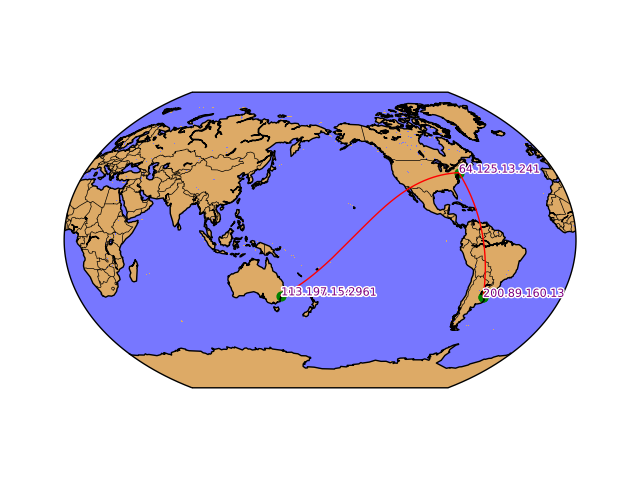
\includegraphics[width=\linewidth]{imagenes/mapa_australia_plotip.png}
		\caption{PlotIP}
		\label{fig:mapa_tsu_plotip}
	\end{subfigure} 
	\begin{subfigure}[b]{0.5\textwidth}
		\centering
		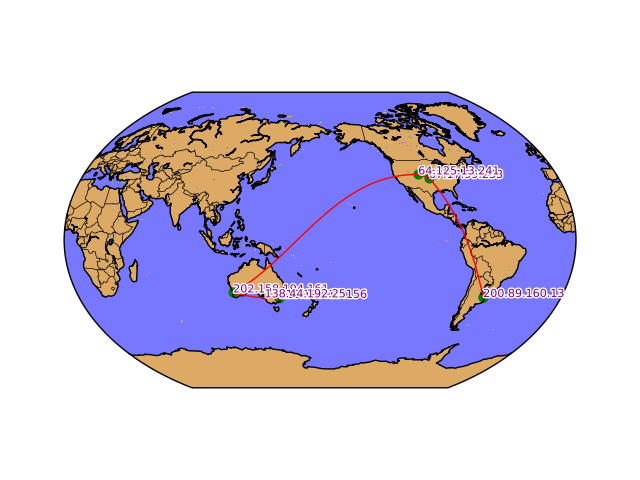
\includegraphics[width=\linewidth]{imagenes/mapa_australia_geoip.png}
		\caption{GeoIPTool}
	\end{subfigure} 
	\caption{Mapas generados a partir de las IP's usando PlotIP/GeoIPTool para la Red de Tecnología Australiana}
	\label{fig:mapas_australia}
\end{figure}

\subsubsection{Round Trip Times}

Para este caso el metodo propuesto nos sugirió dos cables intercontinentales por los que supuestamente se trazo la ruta, uno al saltar a la IP 67.17.99.233 y otro a la IP 202.158.194.161. No obstante en base a las tables y mapas realizados de acuerdo a PlotIP y GeoIPTool, concluimos que la deducción del supuesto salto intercontinental al partir a la IP 67.17.99.233 es un falso positivo, simplemente mal catalogado por ser un salto muy largo que resulto en un relativamente alto RTT. Esta conlusión se sostiene en base a que la IP 67.17.99.233 corresponde a Estados Unidos, y dado que en el medio no parece haber saltado a algun otro continente, lo mas probable sea que simplemente el recorrido de Argentina a Estados Unidos tuvo asociado un $\Delta RTT$ muy alto, lo cual es razonable dado la distacia geografica. A su vez es posible que esto último tambien se deba a la existencia de cables submarinos de larga distancia que van de un punto de América a otro punto del mismo continente, lo cual podría suponer tiempos relativamente altos de propagación tal como ocurre con los cables intercontinentales. Por el contrario el cable intercontinental sugerido al partir a la IP 202.158.194.161, parece concordar con el resto de los datos recabados. Dicha IP es la primera IP de Australia a la que se llega por la ruta obtenida, y dado que el anterior HOP segun los servicios de geolocalización se encuentra en Estados Unidos, el alto $\Delta RTT$ parece tener total sentido debido a que no parece haber habido otra alternativa que la de cruzar un cable intercontinental durante ese tramo para llegar a Australia.

\begin{figure}[ht]\label{fig:rtts_tsu}
	\begin{center}
		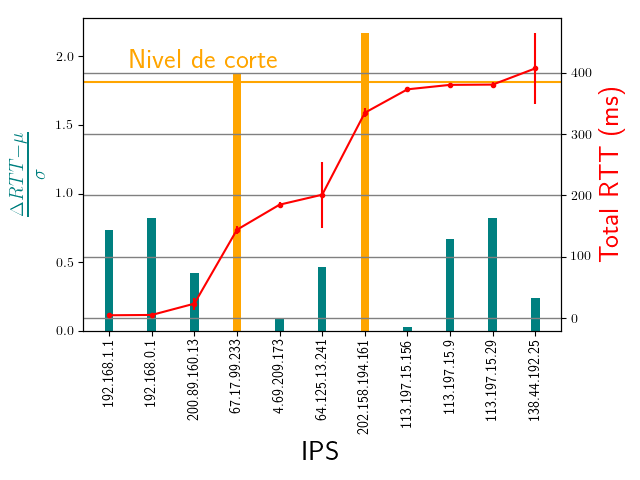
\includegraphics[width=0.8\columnwidth]{imagenes/rtts_australia.png}
		\caption{Grafico de RTTS totales y de enlaces para la Red de Tecnología Australiana}
	\end{center}
\end{figure}

\subsection{Universidad Estatal de Tomsk - Rusia}

En este experimento se analizaron las rutas a la página web
\url{http://www.tsu.ru/} de la Universidad Estatal de Tomsk en Tomsk, Rusía que
en su momento tenía IP 92.63.64.162\footnote{esta IP en el analisis y los
gráficos no aparece debido a que su tiempo de enlace con el gateway anterior
fue negativo}. Durante el monitoreo del experimento se observó que para los
TTL's respondieron Time Exceeded salvo por el ultimo que Respondio Echo Reply.
Además se observo que de los 13 TTLS (de 1 al 13) que respondieron 6 fueron
descartados por tiempos promedios de enlace negativos, dando asi una proporción
de TTL descartados de 46.15\%, que si bien es bastante alta, los resultados
btenidos fueron igual de representativos.


\subsubsection{Posiciones geográficas}

Se observaron las posiciones geográficas como las ciudades y paises segun los
mismos servicios de geolocalizacion que se vienen usando (geoiptool y plotip)
y se observaron las rutas desde Buenos Aires, Argentina hasta Tomsk, Rusia.

Como se puede notar en las tablas \ref{dig:lugares_tsu} la herramienta PlotIP
presentó ciertas rutas anómalas que no se condicen con los tiempos de enlaces
como se puede ver más adelante. Estas posiciones son las de las IP
181.88.170.46, 181.88.109.37 que segun PlotIp se situan en Indonesia,
realizando desde argentina un salto muy grande inexplicable desde los graficos
de los tiempos totales que para esas ips son muy chicos.
Por lo que se concluyó que estos son gateways de Argentina mal clasificados por
PlotIP. Es por esto que se descarta estas IPS (181.88.170.46, 181.88.109.37)
del mapa generado segun PlotIP que se puede ver en la figura
\ref{fig:mapa_tsu_plotip}.

Otro salto poco probable, pero aun no tanto como el anterior, es el de
Belgica-Khabarovsk-Tomsk que cruza desde Bélica, Alemania en Europa hacia
Khabarovsk, Rusia en Asia volviendo a la parte Europea donde se encuentra Tomsk.
Esto es tambien poco contrastable con respecto a los RTTs totales, aunque no tanto
y es por eso que se conservo en el grafico del Mapa (figura \ref{fig:mapa_tsu_plotip}).

Analizando la otra ruta generada a partir de geoiptool esta resulta ser
mas consistente que la que brinda plotip en donde se ve que esta es más directa
y se condice mejor con el grafico de los RTTs.

\begin{figure}[ht]
	\begin{subfigure}[b]{0.5\textwidth}
		\centering
		\begin{tabular}{|c|c|c|c|}
	\hline
	TTL & IP & Ciudad & Pais \\
	\hline
	2 & 200.3.60.22 & Entre Rios & Argentina \\
	\hline
	4 & 181.88.170.46 & & Indonesia \\
	\hline
	5 & 181.88.109.37 & & Indonesia \\
	\hline
	7 & 195.22.214.131 & Bruselas & Bélgica \\
	\hline
	9 & 217.150.44.42 & Khabarovsk & Rusia \\
	\hline
	11 & 82.200.1.210 & Tomsk & Rusia \\
	\hline
\end{tabular}

		\caption{PlotIP}
	\end{subfigure}
	\begin{subfigure}[b]{0.5\textwidth}
		\centering
		\begin{tabular}{|c|c|c|c|}
	\hline
	TTL & IP & Ciudad & Pais \\
	\hline
	2 & 200.3.60.22 & Entre Rios & Argentina \\
	\hline
	4 & 181.88.170.46 & Entre Rios & Argentina \\
	\hline
	5 & 181.88.109.37 & Entre Rios & Argentina \\
	\hline
	7 & 195.22.214.131 &  & Italia \\
	\hline
	9 & 217.150.44.42 &  & Rusia \\
	\hline
	11 & 82.200.1.210 & Tomsk & Rusia \\
	\hline
\end{tabular}

		\caption{GeoIPTool}
	\end{subfigure}
	\caption{Ciudades y Paises de las IP's usando PlotIP/GeoIPTool para la Universidad Estatal de Tomsk - Rusia}
	\label{fig:lugares_tsu}
\end{figure}

\begin{figure}[ht]
	\begin{subfigure}[b]{0.5\textwidth}
		\centering
		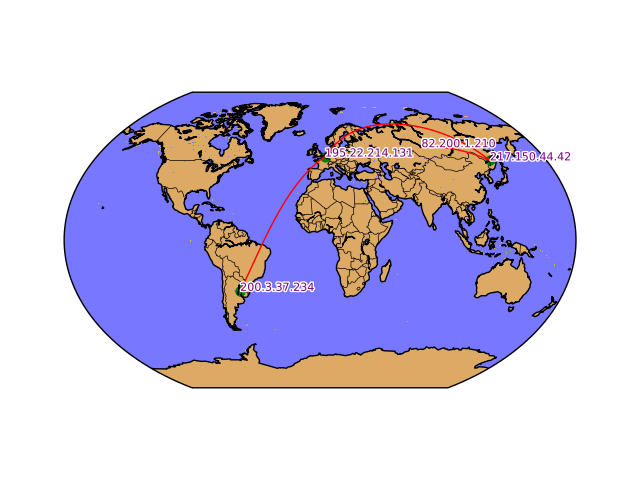
\includegraphics[width=\linewidth]{imagenes/mapa_tsu_plotip.png}
		\caption{PlotIP}
		\label{fig:mapa_tsu_plotip}
	\end{subfigure}
	\begin{subfigure}[b]{0.5\textwidth}
		\centering
		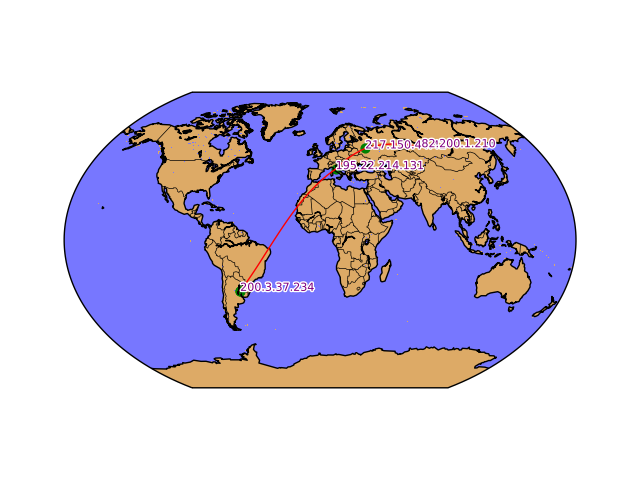
\includegraphics[width=\linewidth]{imagenes/mapa_tsu_geoip.png}
		\caption{GeoIPTool}
	\end{subfigure}
	\caption{Mapas generados a partir de las IP's usando PlotIP/GeoIPTool para la Universidad Estatal de Tomsk - Rusia}
	\label{fig:mapas_tsu}
\end{figure}

\subsubsection{Round Trip Times}

Al analizar los graficos de RTT's que se muestra en la figura
\ref{fig:rtts_tsu} se observa que el método dio un único enlace
intercontinental ya que para ese tamaño de muestra (7) el valor de referencia
de la tabla $t$ se encontraba en 1.71. El gateway que resulta intercontinental
es el 195.22.214.131 y por lo visto anteriormente bien clasificado aun más
siendo este un enlace transatlántico muy posiblemente submarino. El resto de los
tiempos totales son bastante similares ya que como se puede comprobar en el mapa
no son grandes distancias a comparación con la del intercontinental. Finalmente,
en este caso el nivel de aciertos es del 100\% \footnote{Tomsk está considerado
en el contiente européo y no asiático} segun el mapa de geoiptool (que es el que como se mencionó
antes parece equivocarse menos) y por ende no haría falta modificar este valor de
la tabla $t$ ni aplicar ningún criterio de corte ad-hoc para este problema.

\begin{figure}[ht]\label{fig:rtts_tsu}
	\begin{center}
		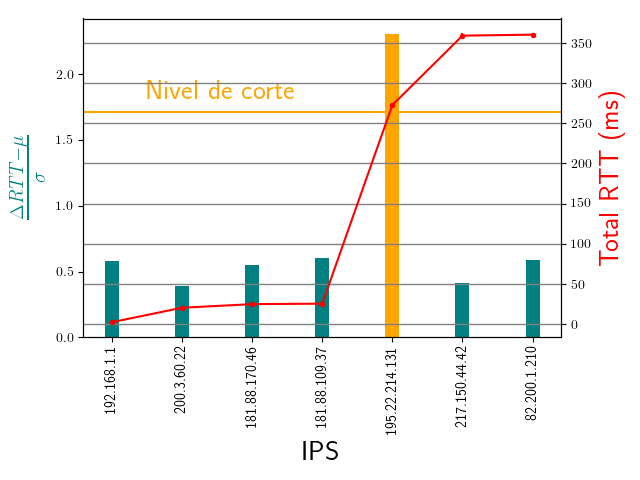
\includegraphics[width=0.8\columnwidth]{imagenes/rtts_tsu.png}
		\caption{Grafico de RTTS totales y de enlaces para la Universidad Estatal de Tomsk - Rusia}
	\end{center}
\end{figure}
